\label{sec:Conducting Matter and Currents}
%%%%%%%%%%%%%%%%%%%%%%%%%%%%%%%
\subsection{Conducting Matter}
A perfect conductor is a macroscopic model for real conducting materials, characterized by the property that static electric fields are completely excluded from its interior. This means that inside a perfect conductor, the electric field is zero, and any charge present is distributed uniformly on the surface of the conductor. The Maxwell equation that underlies this phenomena is Gauss's Law, which relates the divergence of the electric field $E$ to the volumetric charge density $\rho$ via
\begin{equation}
\nabla \cdot E_{in}(r) = \frac{\rho(r)}{\epsilon_0},
\end{equation}
where  $\epsilon_0$ is the permittivity of free space and $\rho(r)$ has units of charge per unit volume. 
\\

Within the volume of the perfect conductor, Gauss's Law shows that the electric field and the charge density must be
\begin{equation}
\label{eq:gausslawconductors}
E_{in}(r) = \rho(r) = 0.
\end{equation}
In fact, this definition ensures that all excess charge accumulates on the surface as surface charge density. Cavendish originally proposed this idea: In the presence of an external field $E_{ext}$  the Coulomb forces rearranges charges inside the metal until the condition in equation \ref{eq:gausslawconductors} is satisfied. This is called polarization and in the general case and \textbf{electrostatic induction} when applied to conductors. 
\begin{figure}[H]
    \centering
    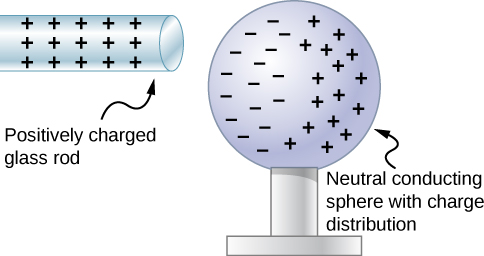
\includegraphics[scale=0.75]{Figures/electricpolarization.jpg}
    \caption{Polarized glass rod and electrostatic induction in sphere.}
    \label{fig:my_label}
\end{figure}

Physicists understand that in the metal, $\rho$ is associated with the electron's quantum mechanical wave functions which spread out over all available atoms. The force density $\rho E_{ext}$ disorts wave functions as to make charges with opposite signs displace in opposite directions \cite{zangwill2013modern}.


\subsection{Currents}
Current continuity equation underlies the conservation of electric charge in current related systems. Mathematically, this equation represents the relationship between current density $j$, and the flow of charge density $\rho$. It is expressed as
\begin{equation}
    \label{eq:continuity}
    \frac{\partial \rho}{\partial t} + \nabla \cdot j = 0, 
\end{equation}
and is derived from Maxwell's equations and plays a crucial role in understanding and analyzing the behavior of electric currents.
\\

In the context of direct currents, charge densities do not change in time so $\nabla \cdot j = 0$. Furthermore, these types of currents create time independent magnetic fields. Thus, the fields of interest satisfy conventional equations of electrostatics which lead to simple, accurate and cheap simulations\footnote{These are good attributes that underlie efficient and use full simulations}.
\\

Current density obey Ohm´s law in the static and time harmonic regime. Such law relates currents to the electric field and the conductivity $\sigma$ by
\begin{equation}
    \label{eq:ohmlaw}
    j = \sigma E.
\end{equation}
This result will be derived in the following section for the time harmonic condition. However, in direct current conditions it is easy to arrive starting from the familiar version of Ohm law
\begin{equation*}
    V=IR=jAR \rightarrow  j = (V/R)/A = \sigma E .
\end{equation*}
You just need to remember that conductivity is the inverse of resistivity and that voltage is related to the electric field. 
\\

\subsection{Drude's Classical Model}
Studying conductivity from a classical point of view provides a very clear physical picture of the phenomena as well as analytical expressions that describe the movement of electrons in conductors! Electron movement is described by a velocity $v(t)$ which is an average measure of how electrons drift through the metal´s atomic lattice and its commonly referred to as \textbf{drift velocity}. This velocity can be related to current and to conductivity as explained in the following paragraphs. 
\\

Start by considering $n$ electrons per unit volume where each one has a charge $q$ and mass $m$. When the conductor is connected to a AC voltage source it generates a time -harmonic electric field $\xi(r,t) = E(r)*exp(-iwt)$ inside the lattice resulting in a time harmonic current. Picture the electron traveling in the crystal structure of a metal (Figure \ref{fig:copper-structure}); the free electrons will eventually collide with atoms in the structure. The mean time of movement before  electrons suffer momentum-degrading collision is called \textbf{relaxation time} $\tau$ \cite{zangwill2013modern}. 
\begin{figure}[H]
    \centering
    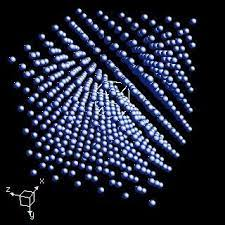
\includegraphics[scale = 0.5]{Figures/copper_structure.jpeg}
    \caption{Copper Crystalline Structure}
    \label{fig:copper-structure}
\end{figure}

Now, pay close attention. Newton´s force laws state that the force on the electrons is given by 
\begin{equation}
    m\frac{dv(t)}{dt}= q * E(r)*e^{-iwt} - \frac{mv(t)}{\tau} \hspace{0.5 cm}[N].
\end{equation}
Time harmonic solutions yield an expression for $v$ of the form
\begin{equation}
    v(t) = \frac{qE/m}{1/\tau -iw} e^{-iwt} = v(w)e^{-iwt} \hspace{0.5 cm}[m/s].
\end{equation}

Current density is formally defined in SI units with $[A/m^2]=[C/m^2s]$. It is simple to see that current density $j$ that develops in the system is given by
\begin{equation}
    \label{eq:current density distribution}
    j(w) = nqv(w) = \frac{nq^2 \tau}{m}\frac{E}{1-iwt} \hspace{0.3 cm}[A/m^2].
\end{equation}
\\

Result in \ref{eq:current density distribution} is then compared to \ref{eq:ohmlaw} to obtain \textbf{Drude´s model of conductivity} where
\begin{equation}
\label{eq:conductivity}
    \sigma(w) = \frac{nq^2 \tau/m}{1-iw\tau} = \frac{\sigma_0}{1-iw\tau} \hspace{0.5 cm}[S/m], 
\end{equation}
is identified as the conductivity of the material; closely related to the current density by Ohm´s law $ j(w) = \sigma(w) E(w)$. As the book \cite{jackson1999classical}, points out, quantum mechanical calculations give the same form for $\sigma$ for simple metals like copper.
\\

\subsection{Regarding Permittivity of Metal}
Permitivity of metal is desscribed by a complex magnitude and should be considered carefully in order to test the validity of crucial aproximations well encounter ahead. 
\cite{jackson1999classical}, continues the discussion by introducing the plasma frequency of the particulhttps://www.overleaf.com/projectar metal, $w_p ^2 = nq^2/\epsilon_0m$ and substuting \ref{eq:conductivity} into (err.find.zanwill.(18.12).  to derive Drude dielectric function,
\begin{equation}
\label{eq:Drude dielectric function}
    \epsilon(w) / \epsilon_0 = [1-\frac{w_p^2 \tau^2}{1+w^2\tau^2}]+i[\frac{w_p^2\tau}{w}\frac{1}{1+w^2\tau^2}]
\end{equation}

\subsection{Regarding Heat effects in currents}
To close this section on conductors with currents, it is worth wile mentioning that current is a process that changes kinetic energy of electrons into heat.  From the first law of thermodynamics (dU = Q-W = 0), the rate of joule heating is equal to the rate at which electric fields does work on the electrons. This phenomena of heat in cables is called joule´s law and is summarized
\begin{equation}
    \frac{dW}{dt} = \frac{d}{dt} \sum q_i E \cdot r = \int d^3r \nabla \cdot (j\phi) = RI^2,
\end{equation}
witch is used when considering thermo-electric effects in cables. 